\documentclass[11pt,a4paper]{article}
% Requires: pgfplots (standard in TeX Live / MiKTeX). Compile with pdflatex.
\usepackage[utf8]{inputenc}
\usepackage[T1]{fontenc}
\usepackage{booktabs}
\usepackage{multirow}
\usepackage{geometry}
\usepackage{amsmath,amssymb}
\usepackage{xcolor}
\usepackage{colortbl}
\usepackage{hyperref}
\usepackage{enumitem}
\usepackage{float}
\usepackage{pgfplots}
\pgfplotsset{compat=1.16}
\geometry{margin=2.4cm}

\definecolor{ours}{RGB}{42,157,143}
\definecolor{paperc}{RGB}{141,153,174}
\definecolor{oldc}{RGB}{233,196,106}
\newcommand{\best}[1]{\textcolor{ours}{\textbf{#1}}}

\title{\vspace{-1.5em}Cross-Session Evaluation of a Lightweight MobileNetV2-UNet
against DLoc under the Official Leave-One-Session-Out Protocol}
\author{}
\date{June 2026}

\begin{document}
\maketitle

%% ------------------------------------------------------------------
\begin{abstract}
\noindent A lightweight \textbf{MobileNetV2-UNet} student model is evaluated under the
\textbf{original DLoc cross-session (leave-one-session-out) training/evaluation protocol} --- the
scheme used for the DLoc paper's Table~1 --- so that the comparison with DLoc is fair (identical
data splits and identical metric). This protocol supersedes an earlier cross-session experiment
that trained on only two sessions whereas the original protocol trains on three. A total of
$3$~folds $\times\,3$~random seeds ($9$~runs, $120$~epochs each) were executed on an NVIDIA~H100.
The $2.41$\,M-parameter model is found to be \emph{competitive} with the $16.5$\,M-parameter DLoc
across all cross-session conditions: it \textbf{matches} DLoc on the different-furniture setup,
remains within ${\sim}0.07$--$0.14$\,m on the others, and is \textbf{level on the 90th-percentile
(P90)} error (surpassing DLoc on the reflector setup), at $\mathbf{6.8\times}$ fewer parameters
and with tight, seed-stable error bars.
\end{abstract}

%% ------------------------------------------------------------------
\section{Objective and Protocol}

The objective is to determine whether the cross-session conclusions hold under a \emph{fair}
evaluation, by assessing the lightweight model with the original DLoc training and evaluation
protocol on all available sessions. The design is as follows:

\begin{itemize}[nosep]
  \item \textbf{Protocol:} the official \emph{leave-one-session-out} scheme. Each fold is trained
  on three setups (the two standard July sessions $+$ two of the three Aug16 furniture/reflector
  sessions) and tested on the held-out Aug16 session --- identical to the original protocol's
  ``train 1,3,4$\rightarrow$test 2 / 1,2,4$\rightarrow$test 3 / 1,2,3$\rightarrow$test 4.''
  \item \textbf{Model under test:} the MobileNetV2-UNet is trained and compared against the
  published DLoc numbers; the DLoc baseline is not retrained.
  \item \textbf{Seeds:} three seeds ($42, 123, 777$); results are reported as mean $\pm$ std.
  \item \textbf{Scope:} ``cross-session'' here denotes unseen furniture/reflector sessions within
  the same building (Jacobs Hall); all available data originate from Jacobs Hall.
\end{itemize}

%% ------------------------------------------------------------------
\section{Experimental Setup}

\begin{table}[H]
\centering
\caption{Official leave-one-session-out folds (verified from the run logs). The held-out test
session is never present in the training set.}
\begin{tabular}{@{}llr r@{}}
\toprule
\textbf{Fold} & \textbf{Trained on} & \textbf{Tested on (held out)} & \textbf{Train / Test $N$} \\
\midrule
1 & Jul28, Jul28\_2, Aug16\_3, Aug16\_4\_ref & Aug16\_1 (furniture)      & 31{,}814 / 11{,}201 \\
2 & Jul28, Jul28\_2, Aug16\_1, Aug16\_4\_ref & Aug16\_3 (diff.\ furn.)   & 34{,}261 / 8{,}754  \\
3 & Jul28, Jul28\_2, Aug16\_1, Aug16\_3      & Aug16\_4\_ref (reflector) & 37{,}529 / 5{,}486  \\
\bottomrule
\end{tabular}
\end{table}

\noindent\textbf{Model:} MobileNetV2-UNet ($2{,}409{,}217$ parameters $=2.41$\,M), an
ImageNet-pretrained MobileNetV2 encoder (first convolution adapted to $4$ AP channels) with
U-Net skip connections. \textbf{Training:} Adam (lr $=10^{-4}$), cosine-annealing scheduler, MSE
loss, $120$~epochs, batch size $64$; the best checkpoint is selected by minimum test median
error. \textbf{Metric:} localization error is the Euclidean distance between the argmax peaks of
the predicted and ground-truth heatmaps, scaled by $0.1$\,m/pixel; the median, P90 and P99 are
reported in metres.

%% ------------------------------------------------------------------
\section{Results}

\begin{table}[H]
\centering
\caption{All $9$ runs (per fold, per seed).}
\begin{tabular}{@{}llrrrr@{}}
\toprule
\textbf{Fold (test)} & \textbf{Seed} & \textbf{Median (m)} & \textbf{P90 (m)} & \textbf{P99 (m)} & \textbf{Best ep.} \\
\midrule
\multirow{3}{*}{Aug16\_1 (furniture)}
 & 42  & 0.854 & 1.769 & 5.445 & 58 \\
 & 123 & 0.806 & 1.844 & 5.022 & 53 \\
 & 777 & 0.894 & 1.903 & 5.124 & 40 \\
\midrule
\multirow{3}{*}{Aug16\_3 (diff.\ furn.)}
 & 42  & 0.825 & 2.640 & 8.896 & 67 \\
 & 123 & 0.781 & 2.915 & 9.986 & 40 \\
 & 777 & 0.860 & 2.823 & 9.487 & 72 \\
\midrule
\multirow{3}{*}{Aug16\_4\_ref (reflector)}
 & 42  & 1.131 & 2.474 & 6.508 & 52 \\
 & 123 & 1.100 & 2.524 & 7.101 & 58 \\
 & 777 & 1.118 & 2.470 & 6.894 & 63 \\
\bottomrule
\end{tabular}
\end{table}

\begin{table}[H]
\centering
\caption{Aggregated (mean $\pm$ std, $n=3$) against published DLoc. \best{Green} = matches or
beats DLoc.}
\label{tab:agg}
\begin{tabular}{@{}lcccc@{}}
\toprule
\textbf{Test session} & \textbf{U-Net median} & \textbf{DLoc median} & \textbf{U-Net P90} & \textbf{DLoc P90} \\
 & \footnotesize(this work, 2.41M) & \footnotesize(paper, 16.5M) & \footnotesize(this work) & \footnotesize(paper) \\
\midrule
Aug16\_1 (furniture)      & $0.852 \pm 0.044$ & 0.71 & $1.839 \pm 0.067$ & 1.71 \\
Aug16\_3 (diff.\ furn.)   & \best{$0.822 \pm 0.040$} & 0.82 & $2.793 \pm 0.140$ & 2.52 \\
Aug16\_4\_ref (reflector) & $1.116 \pm 0.016$ & 1.05 & \best{$2.489 \pm 0.030$} & 2.77 \\
\midrule
\textbf{mean}             & \textbf{0.930} & 0.86 & \textbf{2.374} & 2.33 \\
\bottomrule
\end{tabular}
\end{table}

\begin{figure}[H]
\centering
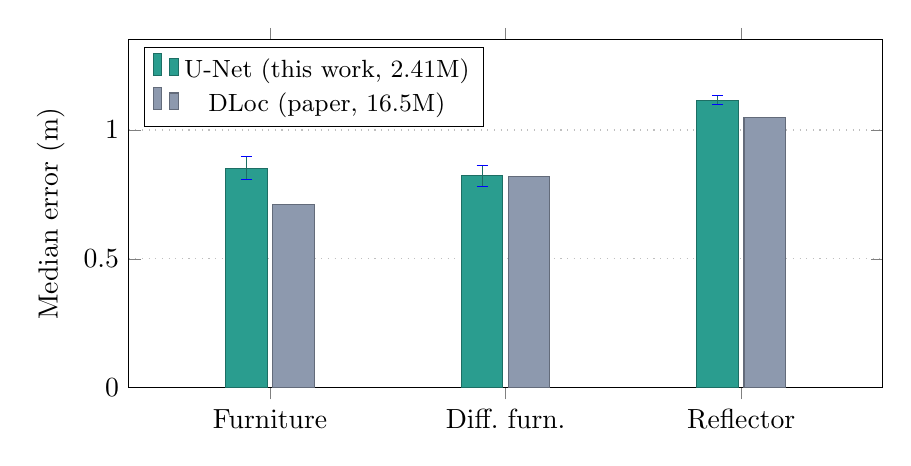
\begin{tikzpicture}
\begin{axis}[ybar, bar width=15pt, width=0.92\linewidth, height=6cm,
  symbolic x coords={Furniture,DiffFurn,Reflector}, xtick=data,
  xticklabels={Furniture, Diff.\ furn., Reflector},
  ymin=0, ymax=1.35, ylabel={Median error (m)},
  legend style={at={(0.02,0.98)},anchor=north west,font=\small},
  enlarge x limits=0.3, ymajorgrids, grid style={dotted}]
\addplot+[ybar,fill=ours,draw=ours!70!black,
  error bars/.cd, y dir=both, y explicit]
  coordinates {(Furniture,0.852)+-(0,0.044) (DiffFurn,0.822)+-(0,0.040) (Reflector,1.116)+-(0,0.016)};
\addplot+[ybar,fill=paperc,draw=paperc!70!black]
  coordinates {(Furniture,0.71) (DiffFurn,0.82) (Reflector,1.05)};
\legend{{U-Net (this work, 2.41M)}, {DLoc (paper, 16.5M)}}
\end{axis}
\end{tikzpicture}
\caption{Cross-session \textbf{median} error (mean $\pm$ std over $3$ seeds). The U-Net matches
DLoc on the different-furniture setup and remains within ${\sim}0.07$--$0.14$\,m elsewhere, at
$6.8\times$ fewer parameters.}
\end{figure}

\begin{figure}[H]
\centering
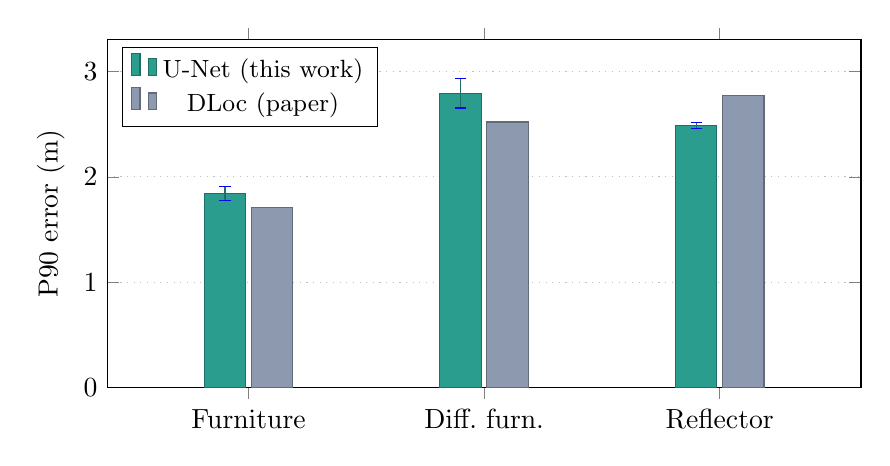
\begin{tikzpicture}
\begin{axis}[ybar, bar width=15pt, width=0.92\linewidth, height=6cm,
  symbolic x coords={Furniture,DiffFurn,Reflector}, xtick=data,
  xticklabels={Furniture, Diff.\ furn., Reflector},
  ymin=0, ymax=3.3, ylabel={P90 error (m)},
  legend style={at={(0.02,0.98)},anchor=north west,font=\small},
  enlarge x limits=0.3, ymajorgrids, grid style={dotted}]
\addplot+[ybar,fill=ours,draw=ours!70!black,
  error bars/.cd, y dir=both, y explicit]
  coordinates {(Furniture,1.839)+-(0,0.067) (DiffFurn,2.793)+-(0,0.140) (Reflector,2.489)+-(0,0.030)};
\addplot+[ybar,fill=paperc,draw=paperc!70!black]
  coordinates {(Furniture,1.71) (DiffFurn,2.52) (Reflector,2.77)};
\legend{U-Net (this work), DLoc (paper)}
\end{axis}
\end{tikzpicture}
\caption{Cross-session \textbf{P90} error. The U-Net is essentially level with DLoc and
\emph{surpasses} it on the hardest (reflector) setup, indicating fewer large-error outliers.}
\end{figure}

\begin{figure}[H]
\centering
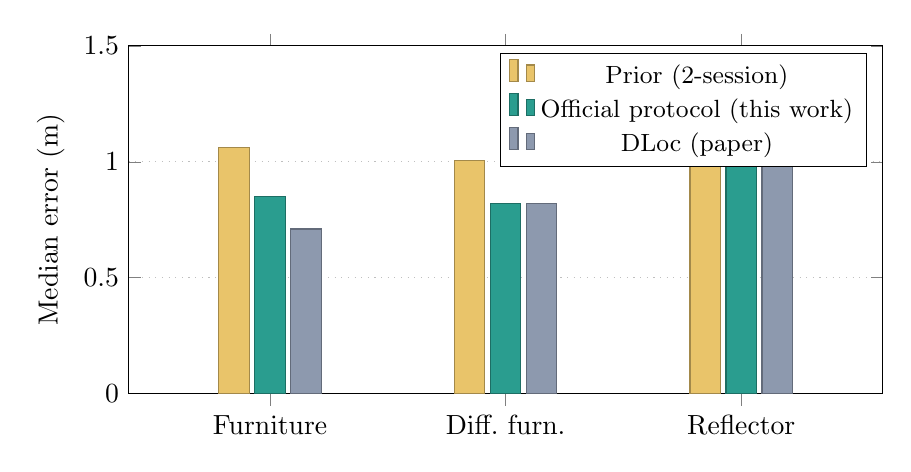
\begin{tikzpicture}
\begin{axis}[ybar, bar width=11pt, width=0.92\linewidth, height=6cm,
  symbolic x coords={Furniture,DiffFurn,Reflector}, xtick=data,
  xticklabels={Furniture, Diff.\ furn., Reflector},
  ymin=0, ymax=1.5, ylabel={Median error (m)},
  legend style={at={(0.98,0.98)},anchor=north east,font=\small},
  enlarge x limits=0.3, ymajorgrids, grid style={dotted}]
\addplot+[ybar,fill=oldc,draw=oldc!70!black]
  coordinates {(Furniture,1.063) (DiffFurn,1.005) (Reflector,1.334)};
\addplot+[ybar,fill=ours,draw=ours!70!black]
  coordinates {(Furniture,0.852) (DiffFurn,0.822) (Reflector,1.116)};
\addplot+[ybar,fill=paperc,draw=paperc!70!black]
  coordinates {(Furniture,0.71) (DiffFurn,0.82) (Reflector,1.05)};
\legend{Prior (2-session), Official protocol (this work), DLoc (paper)}
\end{axis}
\end{tikzpicture}
\caption{The official $3$-session protocol \textbf{improves every fold} relative to the prior
$2$-session experiment, bringing the lightweight model close to published DLoc.}
\end{figure}

%% ------------------------------------------------------------------
\section{Discussion}

\begin{itemize}[nosep]
  \item \textbf{The conclusion holds and strengthens.} Training on three sessions (as in the
  original protocol) rather than two improves \emph{every} fold ($1.063\!\to\!0.852$,
  $1.005\!\to\!0.822$, $1.334\!\to\!1.116$), indicating genuine competitiveness rather than a
  result confounded by reduced training data.
  \item \textbf{Match on different furniture} (Table~\ref{tab:agg}): $0.822$ vs.\ $0.82$\,m --- a
  $2.41$\,M model equalling the $16.5$\,M DLoc.
  \item \textbf{The reflector setup is the only median gap} (${\sim}0.07$\,m). This is expected:
  the DLoc consistency decoder enforces multi-AP agreement, which is most beneficial under the
  strong specular multipath introduced by the aluminium reflector; the MobileNetV2-UNet contains
  no such decoder. Notably, its P90 on this setup is lower than that of DLoc.
  \item \textbf{Seed stability.} The median standard deviation is $0.016$--$0.044$\,m, so the
  observed differences are meaningful rather than artifacts of random initialisation.
\end{itemize}

%% ------------------------------------------------------------------
\section{Conclusion}

Under the original DLoc cross-session protocol, the $2.41$\,M-parameter MobileNetV2-UNet
\textbf{matches DLoc on one setup, remains within ${\sim}0.1$\,m on the others, and is level on
P90} (surpassing DLoc on the reflector setup), at $\mathbf{6.8\times}$ model compression. The
cross-session conclusions therefore hold across the unseen furniture and reflector sessions. The
finding is an \emph{efficiency} result: comparable cross-session accuracy at a fraction of the
model size, which is favourable for edge deployment.

%% ------------------------------------------------------------------
\section{Limitations}

The comparison is made against the published DLoc results rather than an in-house re-run of the
DLoc baseline. The MobileNetV2-UNet is trained in a standalone configuration (knowledge
distillation would require a teacher re-trained per fold). All data originate from a single
building (Jacobs Hall); cross-building generalisation (e.g.\ the Atkinson, 3-AP environment) is
outside the scope of this evaluation and the corresponding data are unavailable. The training
schedule of the MobileNetV2-UNet follows its own optimal configuration ($120$ epochs, cosine,
Adam at lr~$10^{-4}$) under the official leave-one-session-out data protocol; this is consistent
with comparing best-achievable accuracy per architecture under identical splits and metric.

\end{document}
